\chapter{Attaque SSLstrip 2}

\label{sec:sslstrip2}

\begin{figure}[H]
  \caption{Attaque SSLstrip 2 (diagramme Dia)}
  \fbox{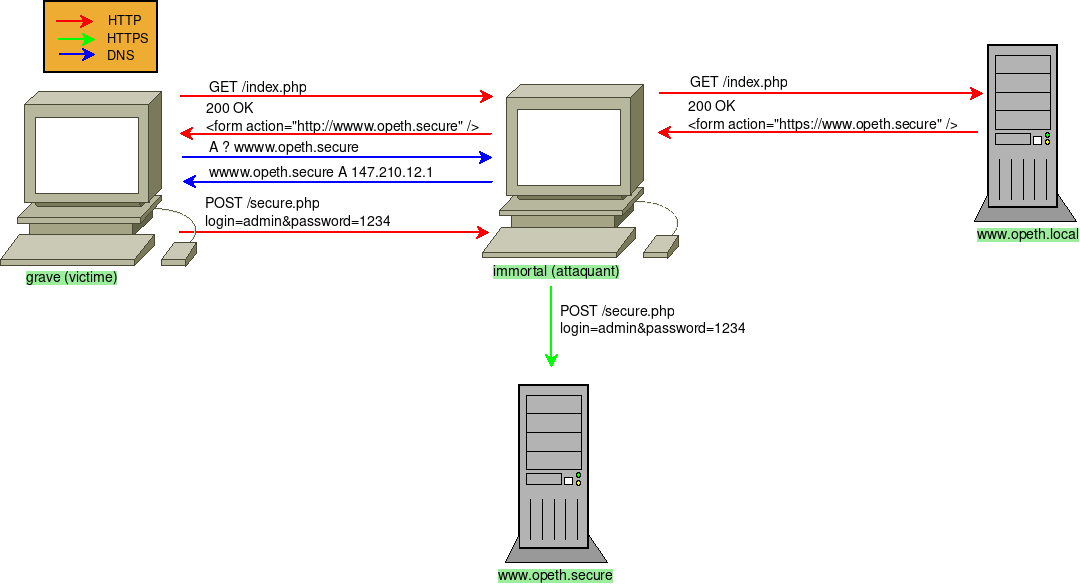
\includegraphics[width=\textwidth]{../medias/sslstrip2/attack.png}}
\end{figure}

Comme vu précédemment, une contremesure a été mise en place afin de déclarer aux clients d'un serveur qu'ils doivent utiliser une connexion sécurisée en HTTPS pour leur futures connexions avec celui-ci. Vous pouvez vous reporter à la section \hyperref[sec:hsts]{Contremesures} pour plus de précision.

Notre but est donc de contourner le HSTS en réutilisant l'attaque SSLStrip. Malheurement, on ne peut pas la réutiliser directement car le navigateur a gardé en que toutes connexions sur cette page doit se faire en HTTPS.

\section{Description de l'attaque}
Cette extension de SSLStrip a été pensée par LeonardoNve. Elle permet donc de passer au travers d'une des nouvelles contremesures mise en place sur les navigateurs. En effet, si l'attaquant se place en homme du milieu, il va pouvoir intercepter le trafic entre le client afin de faire le traiter comme suit.

Lorsque le client va se connecter au serveur sur une page HTTP, l'attaquant va modifier sur cette page en remplaçant tous les liens HTTPS en HTTP mais aussi en changeant le nom de domaine. Changer le nom de domaine changera le comportement du navigateur. En effet, comme le navigateur ne connaît pas ce nom de domaine, il n'envera pas d'exception.

Voici un exemple :

Si le lien est \path{https://www.domain.secure} , on peut le remplacer par \path{http://wwww.domain.secure}.

Il faut noté que l'on enlève le \verb+s+ de \verb+https+ et que l'on remplace \verb+www+ par \verb+wwww+ ce qui change bien le nom de domaine.

Ainsi, l'attaquant fait croire au navigateur que cette requête est légitime et que \path{wwww.domain.secure} correspond au serveur distant. La connexion sera donc en HTTP, donc en clair.

\section{Notre attaque}

Tout d'abord, afin de pouvoir mettre en place l'attaque, il nous faut configurer l'environnement. Rappelons que l'attaquant est déjà positionné en homme du milieu, et que nous avons choisi de mettre sa machine dans le même réseau que la machine victime. Comme pour l'attaque précédente, nous utilisons l'outil \verb+qemunet+ développer par l'Inria qui nous permet de créer un environnement minimaliste et léger. Il nous faut donc vous expliquer sa mise en place.

\subsection{Mise en place de l'environnement}

Dans un premier temps, nous devons créer une topologie, c'est à dire un fichier d'écrivant l'architecture de l'environnement, qui correspond à notre besoin. En effet, nous avons besoin de trois machines:

\begin{itemize}
\item une machine cliente et victime
\item une machine attaquante
\item une machine serveur
\end{itemize}

% mettre une capture de la topologie

Afin d'utiliser \verb+qemunet+ facilement, nous avons décidé de structurer l'environnement de l'attaque grâce à la gestion de dossier supportée par l'outil. C'est pourquoi, tout l'environnement de l'attaque se trouve dans le dossier \verb+sslstrip2+ de notre projet. Ce dossier étant lui-même réparti en sous-dossier. Chaque sous-dossier représente chaque machine :

\begin{itemize}
\item grave : dossier de la machine cliente et victime
\item immortal : dossier de la machine attaquante
\item opeth : dossier de la machine serveur
\end{itemize}

De plus, afin d'avoir une configuration qui est chargée à chaque lancement du système, nous utilisons des scripts bash \verb+start.sh+ qui sont chargés par \verb+qemunet+ au démarrage de chaque machine.

Maintenant, il nous faut décrire ces fichiers de lancement.

\subsubsection{Configuration de la machine cliente}
Cette machine se nomme grave et utilse un environnement graphique de la distribution Linux Alpine. Un navigtateur Firefox est présent pour la démonstration ultérieure.

Pour que la machine puisse accéder au réseau internet, nous devons lui spécifier une addresse IP ainsi que son masque de sous-réseau, sa route par défaut.

Mais, dans le cadre de l'attaque, il faut aussi les informations pour la résolution du nom de domaine en rapport avec l'adresse IP du serveur. Nous en reparlerons plus en détail ultérieurement.

De plus, comme nous allons utiliser du HTTPS, il nous a fallût créer des certificats reconnus par le navigateur client. Pour cela, il nous est nécessaire d'ajouter le certificat dans les fichiers configuration de Firefox afin qu'il le considère comme de confiance.

\inputminted[bgcolor=lbcolor, breaklines]{shell}{../sslstrip2/grave/start.sh}

\subsubsection{Configuration de la machine serveur}

\subsubsection{Configuration de la machine attaquante}

\subsubsection{Mise en place du DNS}

\subsection{Explication du code}

\subsection{Démonstration}
